\documentclass[article]{ajs}

%%%%%%%%%%%%%%%%%%%%%%%%%%%%%%
%% declarations for jss.cls %%%%%%%%%%%%%%%%%%%%%%%%%%%%%%%%%%%%%%%%%%
%%%%%%%%%%%%%%%%%%%%%%%%%%%%%%

\usepackage{wrapfig}
\usepackage{graphicx}

%% almost as usual
\author{Sebastian Warnholz\\ Freie Universit\"at Berlin \And 
        Timo Schmid \\ Freie Universit\"at Berlin}
\title{Simulation Tools for Small Area Estimation: Introducing the \proglang{R}-package \proglang{saeSim}}

%% for pretty printing and a nice hypersummary also set:
\Plainauthor{Sebastian Warnholz, Timo Schmid} %% comma-separated
\Plaintitle{Simulation Tools for Small Area Estimation: Introducing the R-package saeSim} %% without formatting
\Shorttitle{Simulation Tools for Small Area Estimation} %% a short title (if necessary)

%% an abstract and keywords
\Abstract{
  The abstract of the article in English
  
}
\Keywords{package, small area estimation, reproducible research, simulation, \proglang{R}}
\Plainkeywords{package, small area estimation, reproducible research, simulation, R} %% without formatting
%% at least one keyword must be supplied

%% publication information
%% NOTE: Typically, this can be left commented and will be filled out by the technical editor
%% \Volume{50}
%% \Issue{9}
%% \Month{June}
%% \Year{2012}
%% \Submitdate{2012-06-04}
%% \Acceptdate{2012-06-04}
%% \setcounter{page}{1}
\Pages{1--xx}

%% The address of (at least) one author should be given
%% in the following format:
\Address{
  Sebastian Warnholz\\
  Department of Economics\\
  Freie Universit\"at Berlin\\
  D-14195 Berlin, Germany\\
  E-mail: \email{Sebastian.Warnholz@fu-berlin.de}\\
  URL: \url{http://www.wiwiss.fu-berlin.de/fachbereich/vwl/Schmid/Team/Warnholz.html}
}
%% It is also possible to add a telephone and fax number
%% before the e-mail in the following format:
%% Telephone: +43/512/507-7103
%% Fax: +43/512/507-2851

%% for those who use Sweave please include the following line (with % symbols):
%% need no \usepackage{Sweave.sty}

%% end of declarations %%%%%%%%%%%%%%%%%%%%%%%%%%%%%%%%%%%%%%%%%%%%%%%


\begin{document}

%% include your article here, just as usual

% R CMD Sweave %.Rnw
% Loading (and installing) necessary packages.

\section{Introduction}
Reproducible Research has become a widely discussed topic inside science and also the field of statistics. Thanks to the many mostly open-source tools like the \proglang{R}-language and \LaTeX, and also packages like knitr and Sweave, the integration of source code and text is possible and as a problem solved. In that sense the demand for Literate Programming can be if wanted incorporated in the work flow of a scientist. Not only are tools available to make research reproducible, also the demand of making the analysis of articles reproducible is rising. What this means is, that the source-code and data is published alongside an article. However, the requirements in style and clarity of source code are different from the written words in the article itself. This demand \textit{human readable source-code} has already been expressed by Knuth (1984): 
\begin{quote}
\textit{Instead of imagining that our main task is to instruct a computer what to do, let us concentrate rather on explaining to human beings what we want a computer to do.}
\end{quote}
Small Area Estimation is a growing field inside the field of statistics, where simulation studies play an important role. New statistical models are applied in model-based and design-based simulation studies. Considering the demands in reproducibility we want to propose a framework for simulation studies. This framework addresses three demands. First, making tools for data generation available and reusable. Second, unify the process behind simulation studies inside the field of Small Area Estimation. And third, making source-code of simulation studies available, such that it supports the conducted research in a transparent manner.
In this article we want to introduce a new package for the \proglang{R}-language addressing these demands. We will show the importance of simulation studies in the field. Introduce the simulation framework. And demonstrate how to use the package to map the simulation as a process to \proglang{R}.

\section{Small Area Estimation}
What is small area estimation? 2 Models to introduce. FH + BHF. Why are simulation studies important in the field.


\section{A simulation framework}

%% flow-diagram
\begin{wrapfigure}{R}{0.5\textwidth}
\begin{center}
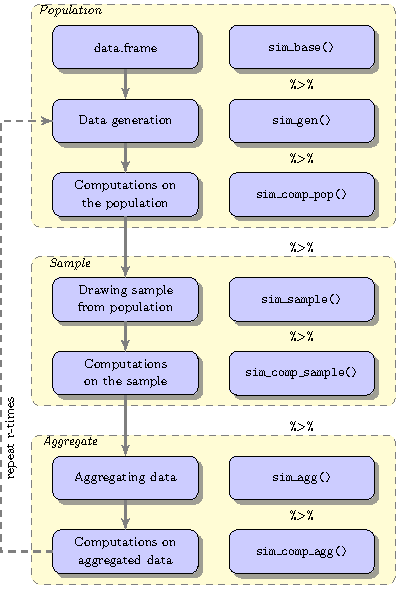
\includegraphics[width=0.5\textwidth]{flowdiagram}
\end{center}
\caption{\label{fig:flowdiagram}Process of simulation.} 
\end{wrapfigure}

Design- vs. model-based simulation, we do not promote one or the other. 
Figure \ref{fig:flowdiagram} illustrates the steps in a simulation. Based on a data table, which may be a real or synthetic population or a set of ID variables representing the hierarchy of the data, you start a simulation.

Introducing a simulation study as a data manipulation process. From data generation to estimating models. How can this process be mapped into the \proglang{R}-language. Present the simulation phases as flow-diagram and map the function names to the problem domain. Defining interfaces between phases: \proglang{data.frame} in, \proglang{data.frame} out. What is the difference between a design-based (fixed-population) and model-based (random-population) approach. 

Why is this package helping in terms of literate programming (code is written for humans not machines) and reproducible research? Package naming conventions. Use the \proglang{\%>\%} operator to compose simulation set-ups. Reuse defined scenarios to compose new scenarios: What is a contamination scenario? A standard scenario plus contamination:

asd asd asd asd asd asd asd asd asd asd asd asd asd asd asd asd asd asd asd asd asd asd asd asd asd asd asd asd asd asd asd asd asd asd asd asd asd asd asd asd asd asd asd asd asd asd asd asd asd asd asd asd asd asd asd asd asd asd asd asd asd asd asd asd asd asd asd asd asd asd asd asd asd asd asd asd asd asd asd asd asd asd asd asd asd asd asd asd asd asd asd asd asd asd asd asd asd asd asd asd asd asd asd asd asd asd asd asd asd asd asd asd asd asd asd asd asd asd asd asd asd asd asd asd asd asd asd asd asd asd asd asd asd asd asd asd asd asd asd asd asd asd asd asd asd asd asd asd asd asd asd asd asd asd asd asd asd asd asd asd asd asd asd asd 

\begin{Schunk}
\begin{Sinput}
> contaminatedSetup <- standardSetup %>% sim_gen_cont()
\end{Sinput}
\end{Schunk}

First develop a scenario outside any looping structures, then run it R-times:

\begin{Schunk}
\begin{Sinput}
> simulationResults <- simSetup %>% sim(R = 500)
\end{Sinput}
\end{Schunk}

There is an easy back-end to run simulations in parallel (in Windows with special care):

\begin{Schunk}
\begin{Sinput}
> simulationResults <- simSetup %>% sim(R = 500, parallel = TRUE)
\end{Sinput}
\end{Schunk}

\section{Data generation}
This is not a data generation tool. However, it supports some useful functions to add random variates to the data. Definition of outliers, see Rao (?) -- how is it addressed in the package. More than linear models, define any response with:
\begin{Schunk}
\begin{Sinput}
> setup %>% sim_resp_eq(y = g(2 * x) + e)
\end{Sinput}
\end{Schunk}

\section{Adding steps to a simulation}
Is present in unit-level simulation studies. Draw with simple random sampling from the whole population or within cluster/domains. Specify the sample size as integer or fraction and add weights if necessary. Wrappers around \proglang{dplyr::sample\_n} and \proglang{dplyr::sample\_frac}.
Adding user specified functions to the simulation process is what separates this package from a mere data generation tool. The interface is simple: Add functions with one argument which is the data at that moment and which return the modified data. I am not sure if this and the sampling section is necessary -- maybe it should just be summarized in the overview section...

\section{Case study}

\section{Outlook}
Use this package to share and publish simulation studies alongside papers. Contribute to the package to make your ideas available. Contribute to the package and make your whole simulation study available. 


%\bibliographystyle{plainat}
\bibliography{saeSim}



\end{document}
